% \subsubsection{Code snippets}

% https://tex.stackexchange.com/questions/542803/removing-blank-pages
% \let\cleardoublepage=\clearpage
\subsection*{Additional figures}
\addcontentsline{toc}{subsection}{\protect\numberline{}Additional figures}

\begin{figure}
    \vspace{-50px}
    \centering
    \caption{Project Timeline}
    \label{fig:ProjectTimeline}
    \begin{subfigure}[t]{0.5\textwidth}
        \caption{Timeline table}
        \label{fig:ProjectTimelineChart}
        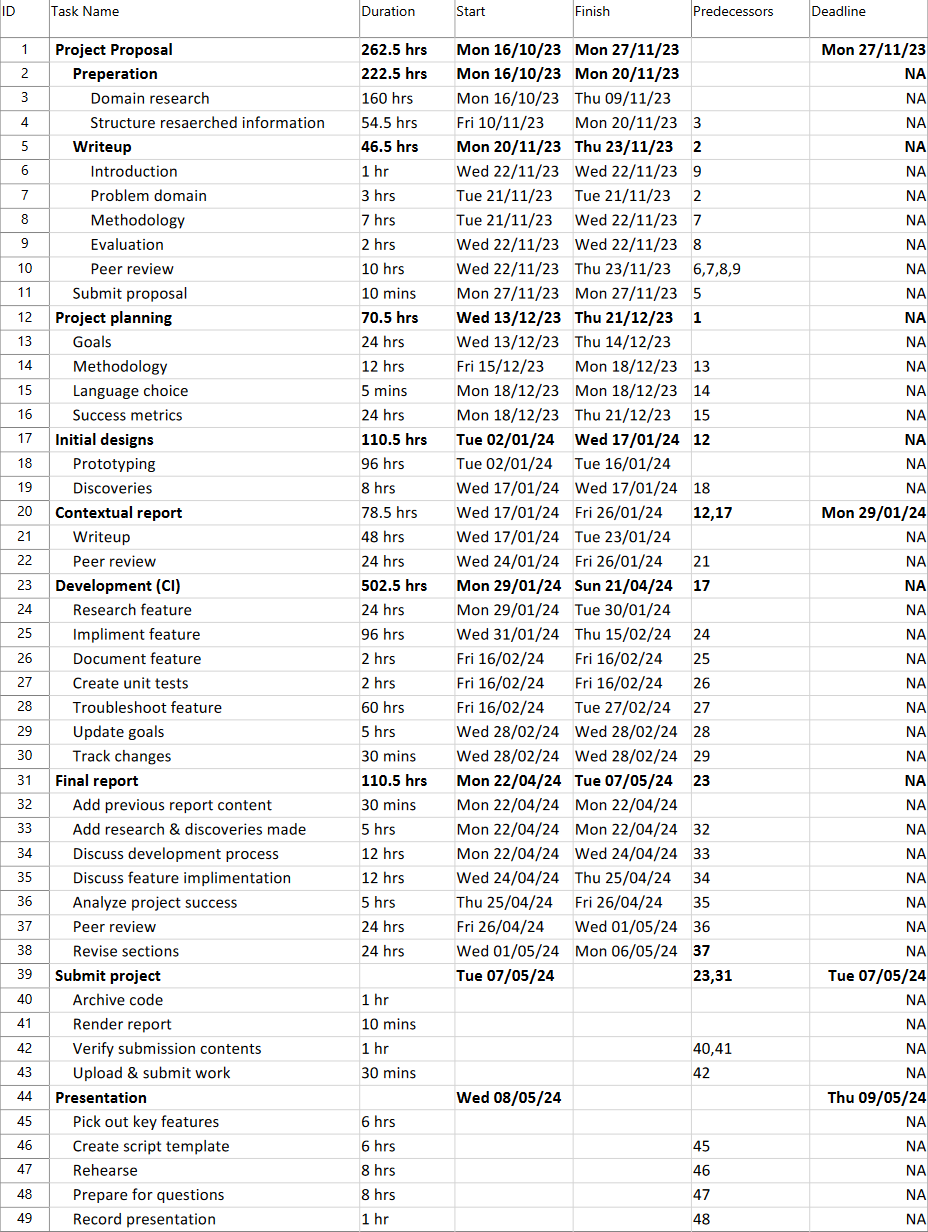
\includegraphics[width=0.5\textheight]{Figures/TimelineChart.png}
    \end{subfigure}
    % \vspace{10px}
    \begin{subfigure}[b]{1.0\textwidth}
        \vspace{10px}
        \caption{Gantt chart}
        \label{fig:GanttChart}
        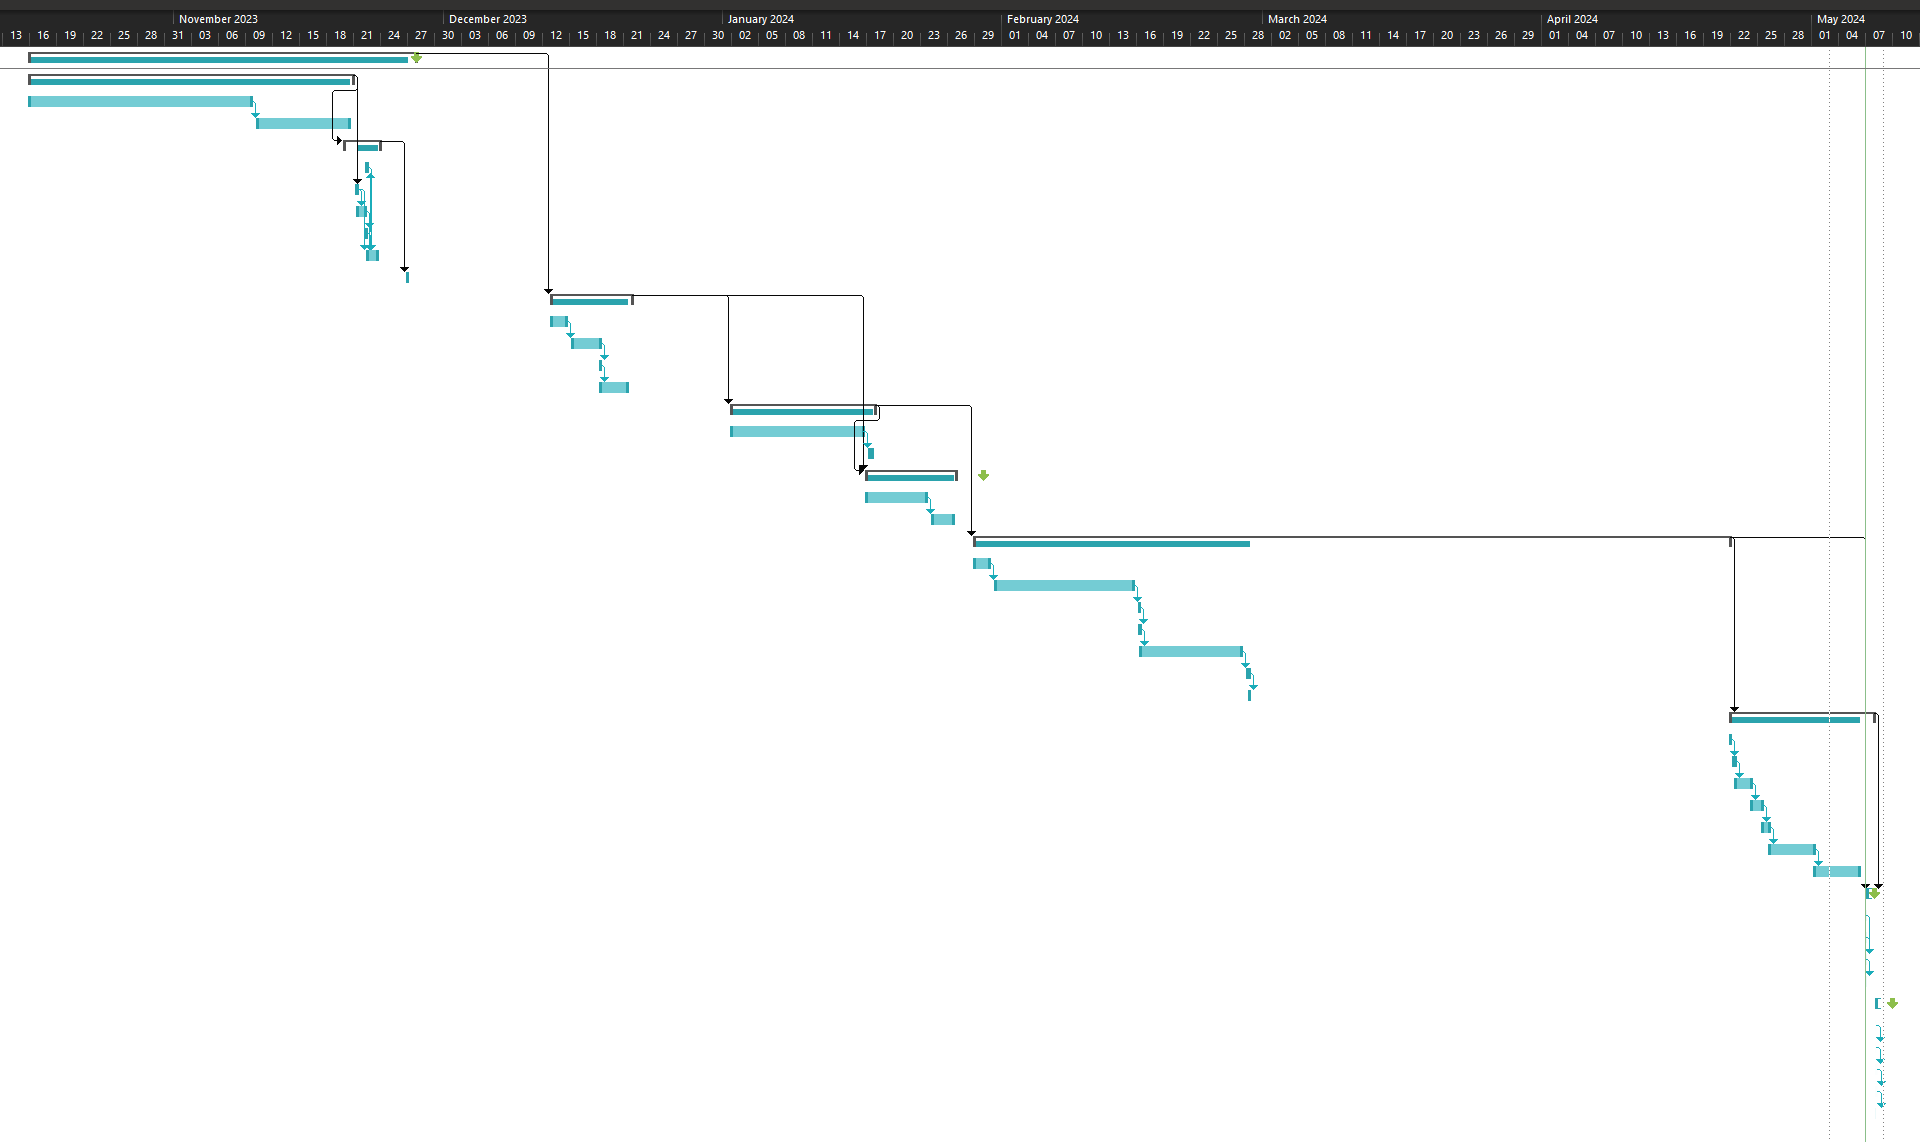
\includegraphics[width=1.0\textwidth, height=0.3\textheight]{Figures/GanttChart.png}
    \end{subfigure}
\end{figure}

\begin{figure}\centering\makebox[\textwidth][c]
{
    \begin{minipage}[t]{0.6\linewidth}
        \vspace{-75px}
        \centering
        \caption{Using GitHub to track changes and issues}
        \label{fig:GitCommitHistory}
        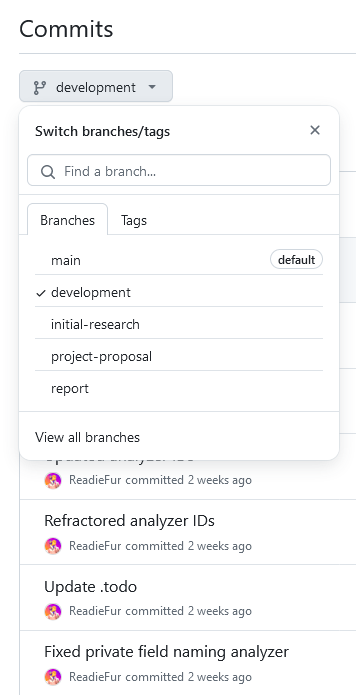
\includegraphics[width=\linewidth, height=0.4\textheight, keepaspectratio]{Figures/GitHubCommitHistoryCropped.png}
    \end{minipage}
    \begin{minipage}[t]{0.65\linewidth}
        \vspace{-75px}
        \centering
        \caption{YAML Schema}
        \label{fig:YAMLSchema}
        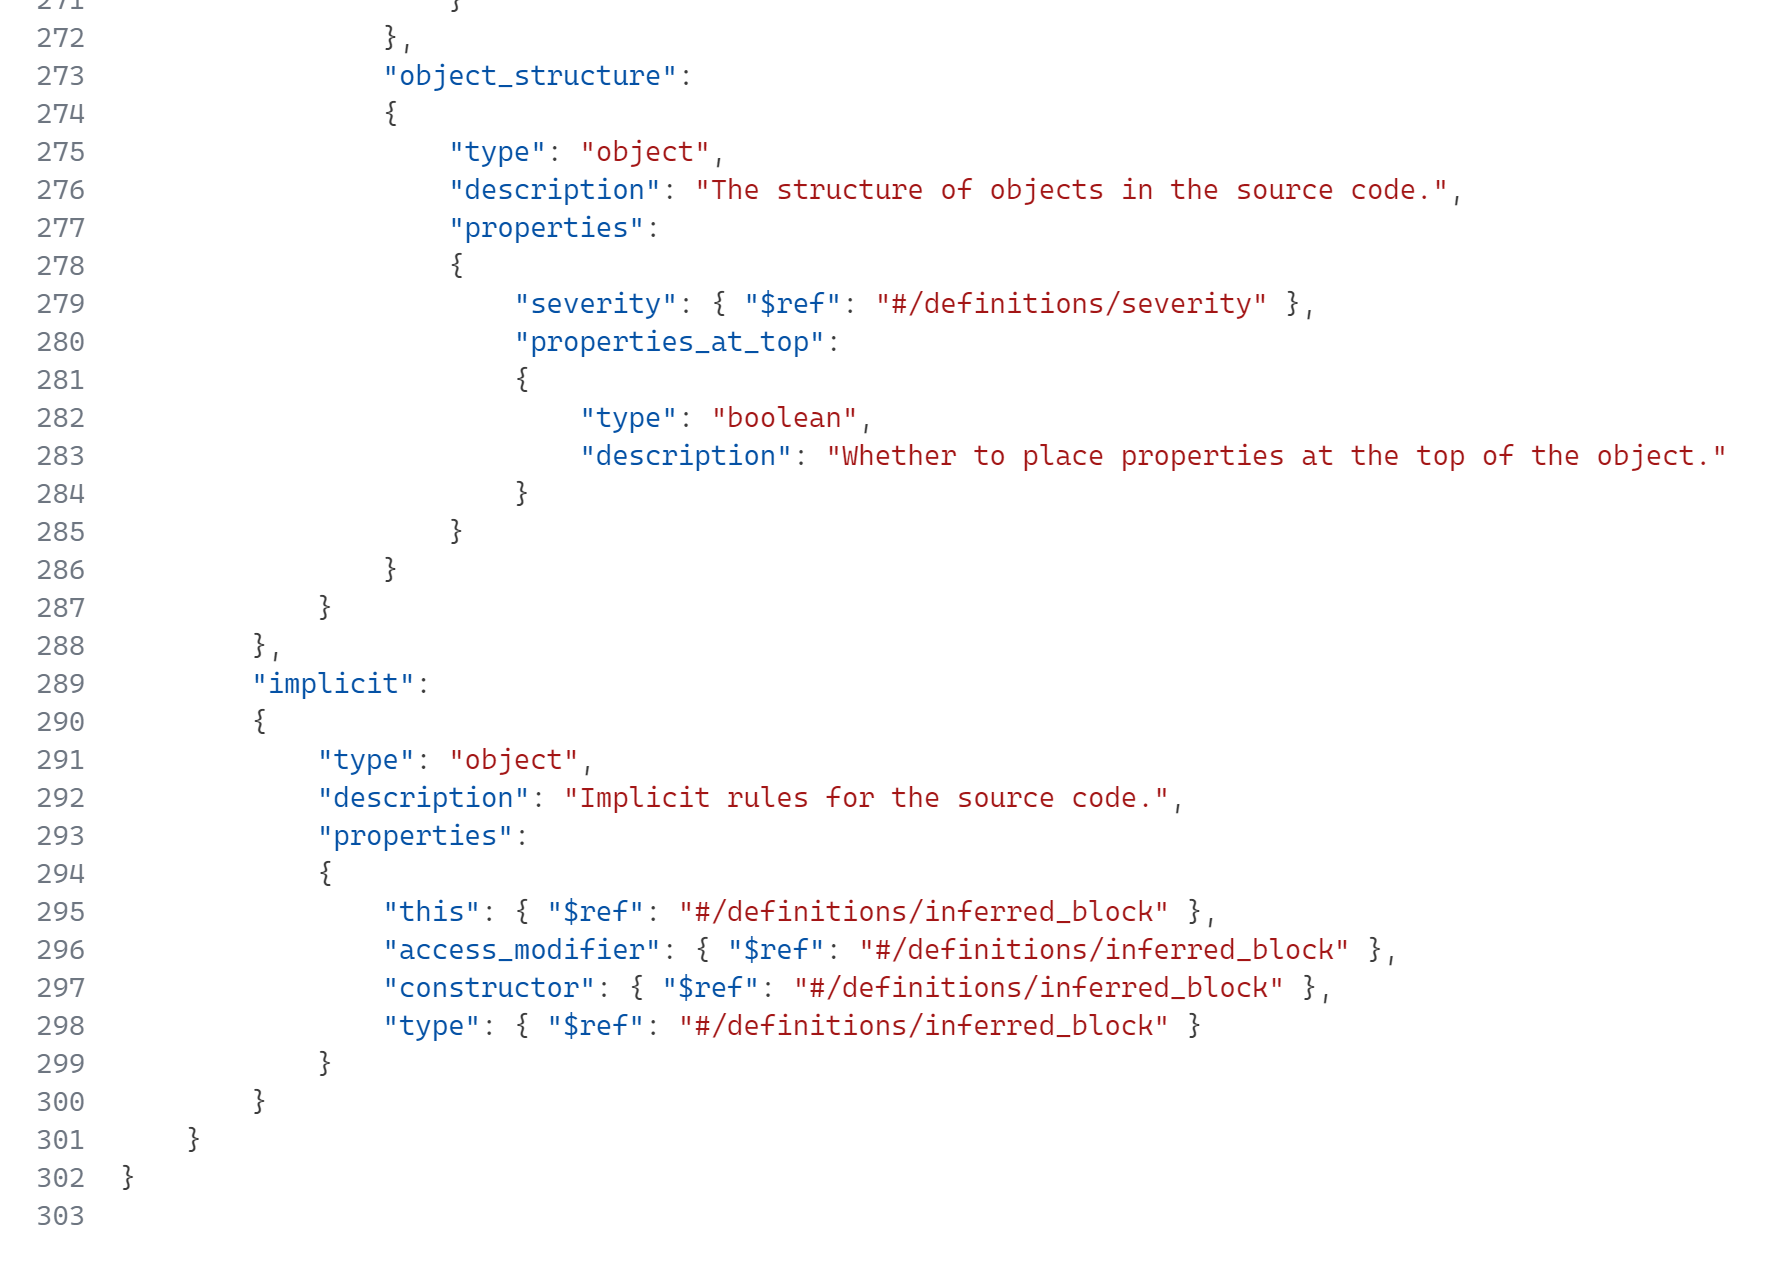
\includegraphics[width=\linewidth, height=\textheight, keepaspectratio]{Figures/YAMLSchemaCropped.png}
    \end{minipage}
}
\end{figure}

% \begin{figure}
%     % \vspace{-35px}
%     \centering
%     \caption{Using GitHub to track changes and issues}
%     \label{fig:GitCommitHistory}
%     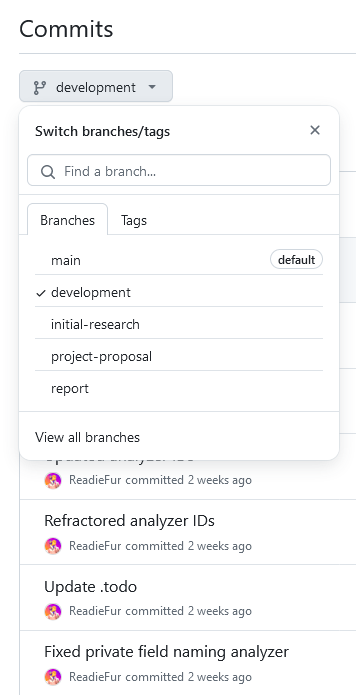
\includegraphics[width=0.25\textwidth]{Figures/GitHubCommitHistoryCropped.png}
% \end{figure}

% \begin{figure}
%     % \vspace{-50px}
%     \centering
%     \caption{YAML Schema}
%     \label{fig:YAMLSchema}
%     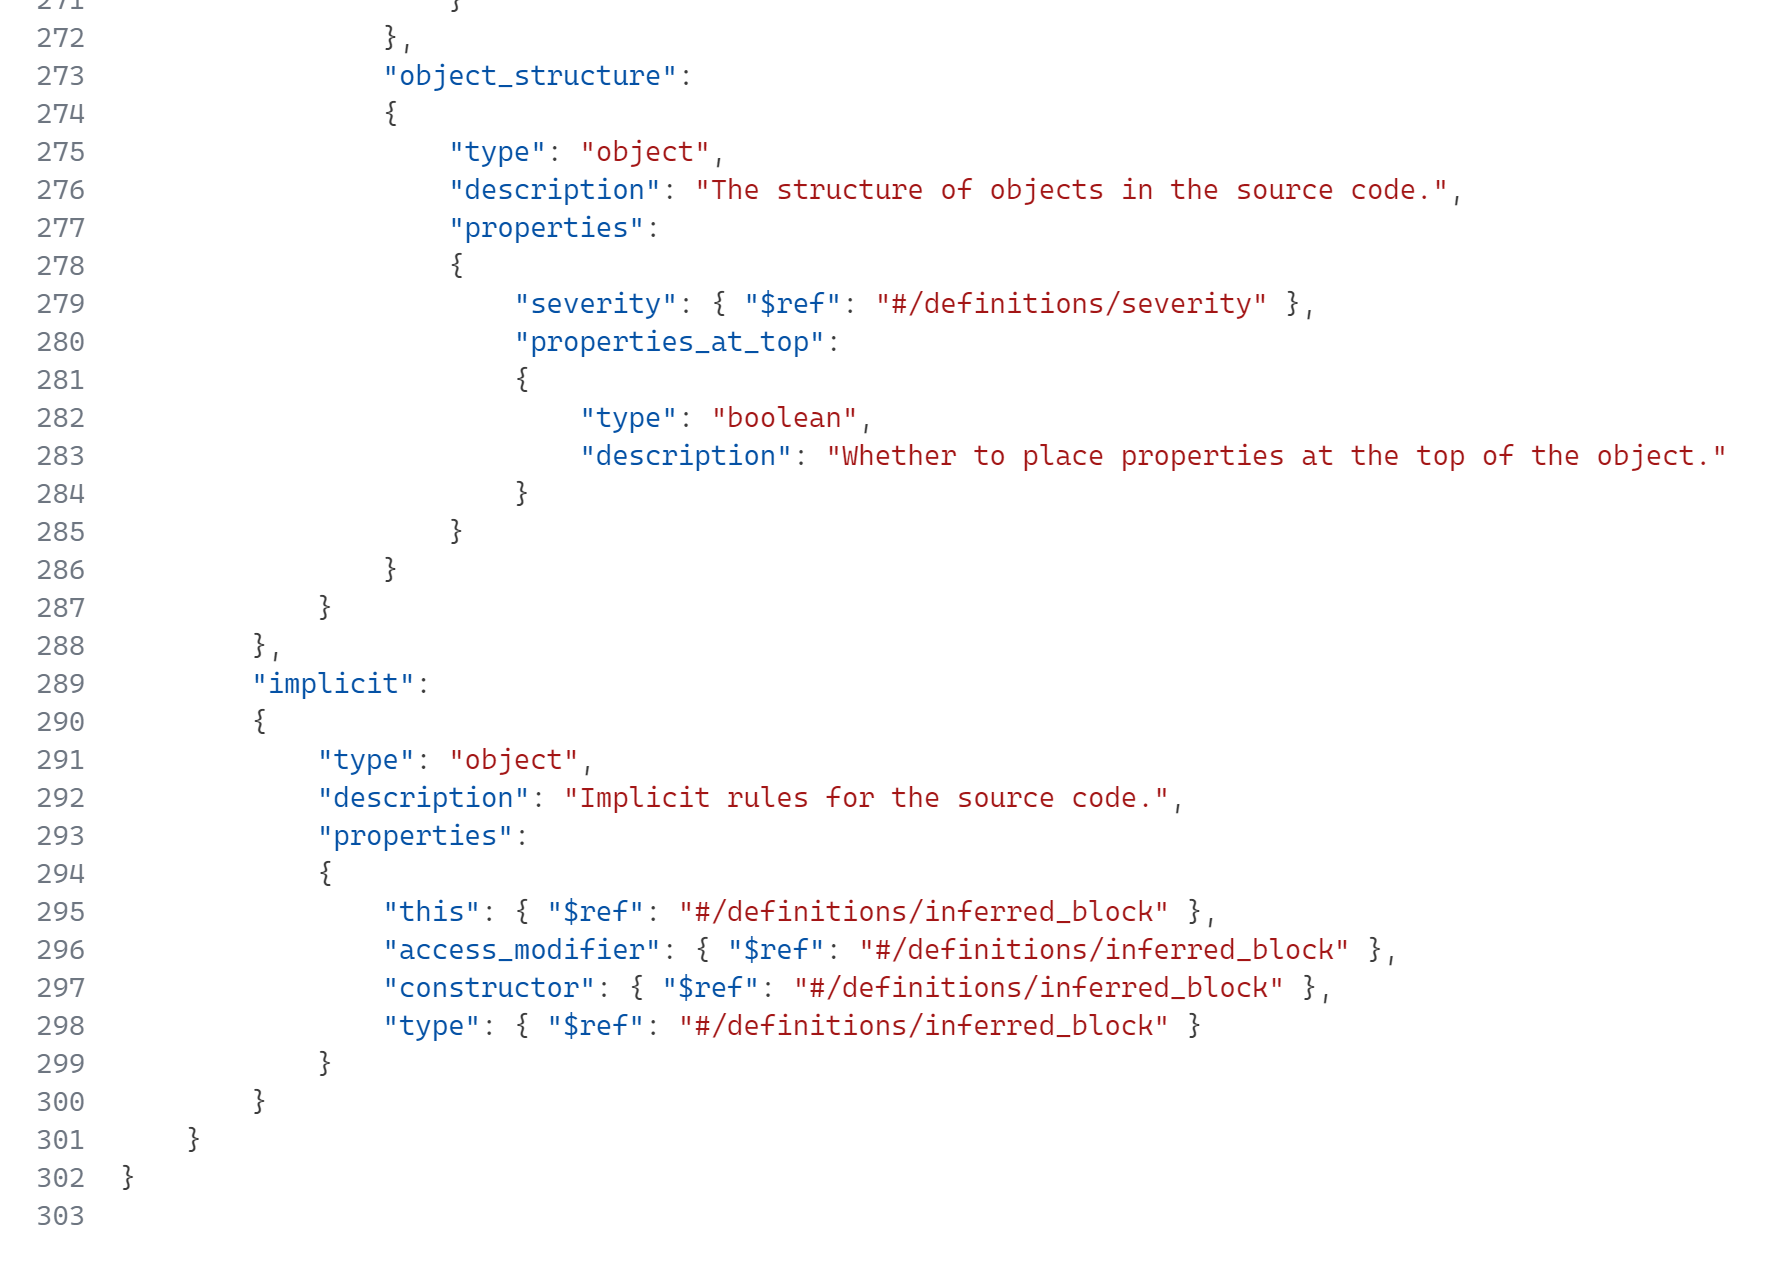
\includegraphics[width=0.5\textwidth]{Figures/YAMLSchemaCropped.png}
% \end{figure}

% \begin{figure}
%     \caption{Regex Token Recursive Parse}
%     \label{fig:RegexTokenRecursiveParse}
%     \centering
%     \begin{subfigure}[b]{0.5\textwidth}
%         \caption{Group Construct Recursive Parse}
%         \label{fig:GroupConstructRecursiveParse}
%         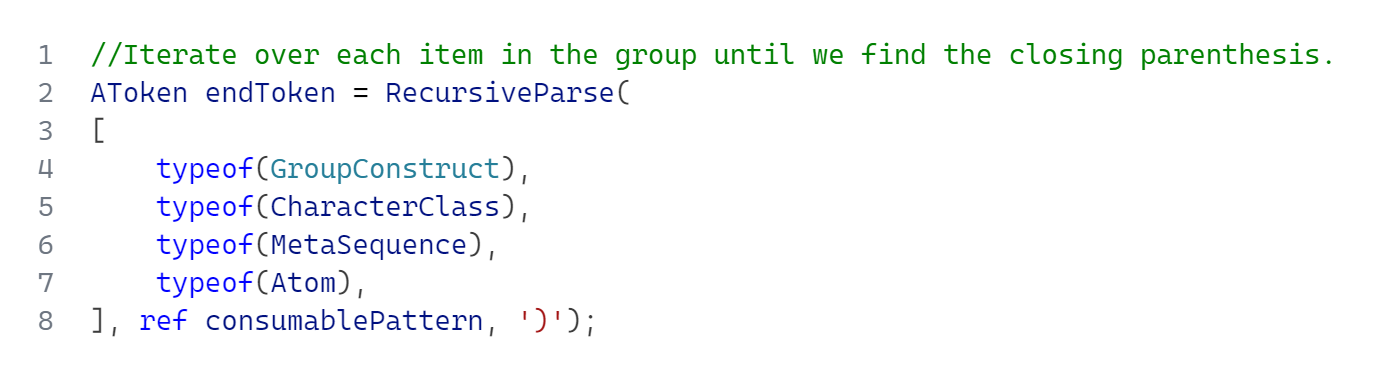
\includegraphics[width=\linewidth, height=0.3\textheight, keepaspectratio]{Figures/GroupConstructRecursiveParse.png}
%     \end{subfigure}
%     \begin{subfigure}[b]{0.5\textwidth}
%         \caption{Recursive Token Parser}
%         \label{fig:AToken_RecursiveParse}
%         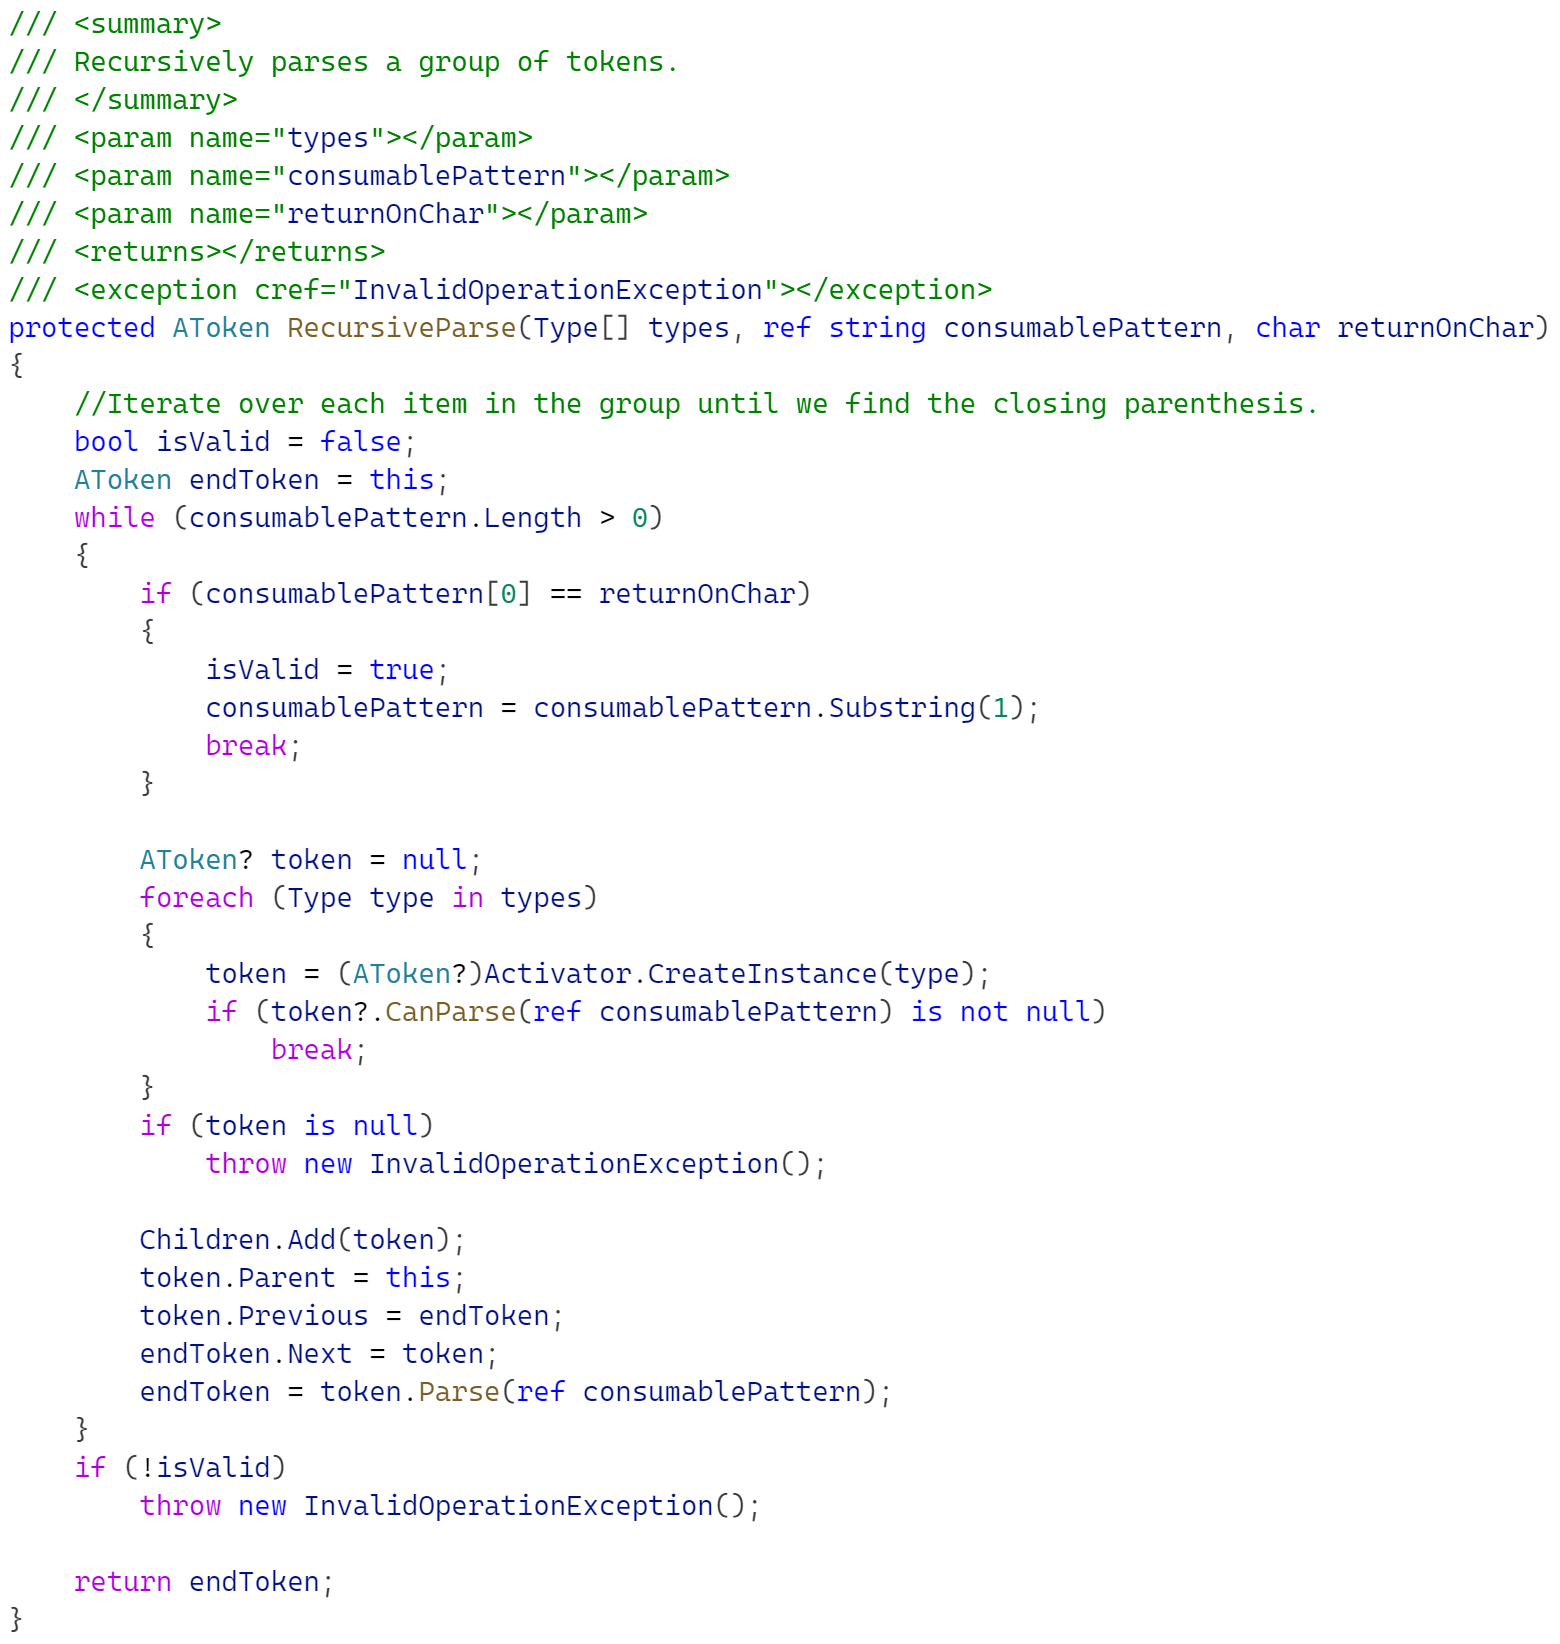
\includegraphics[width=\linewidth, height=\textheight, keepaspectratio]{Figures/AToken_RecursiveParse.png}
%     \end{subfigure}
% \end{figure}

% \vspace{20px}
\begin{figure}\centering\makebox[\textwidth][c]
{
    % \vspace{20px}
    \begin{minipage}[t]{0.6\linewidth}
        % \vspace{20px}
        % \vspace{-100px}
        \caption{Regex Token Recursive Parse}
        \label{fig:RegexTokenRecursiveParse}
        \centering
        \begin{subfigure}[b]{0.9\linewidth}
            \caption{Group Construct Recursive Parse}
            \label{fig:GroupConstructRecursiveParse}
            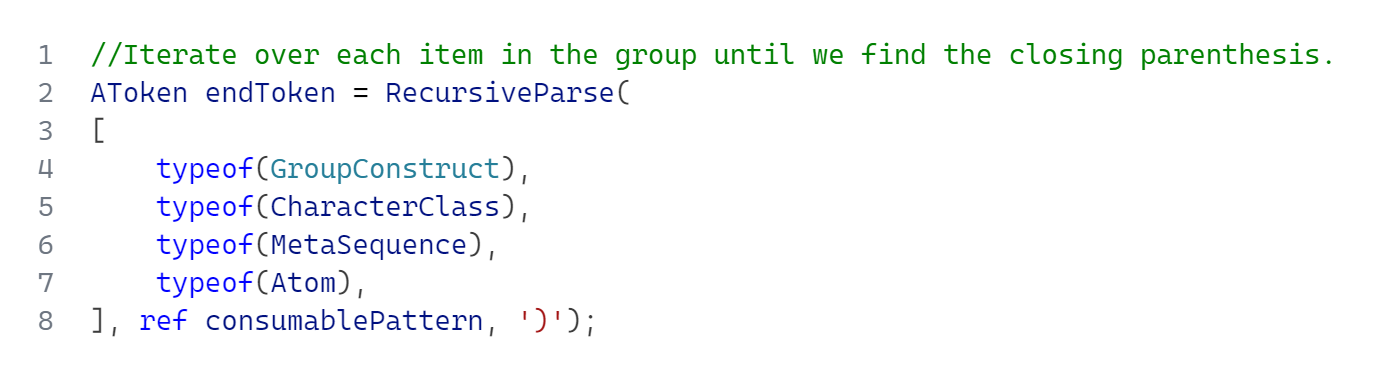
\includegraphics[width=\linewidth, height=0.3\textheight, keepaspectratio]{Figures/GroupConstructRecursiveParse.png}
        \end{subfigure}
        \begin{subfigure}[b]{0.9\linewidth}
            \caption{Recursive Token Parser}
            \label{fig:AToken_RecursiveParse}
            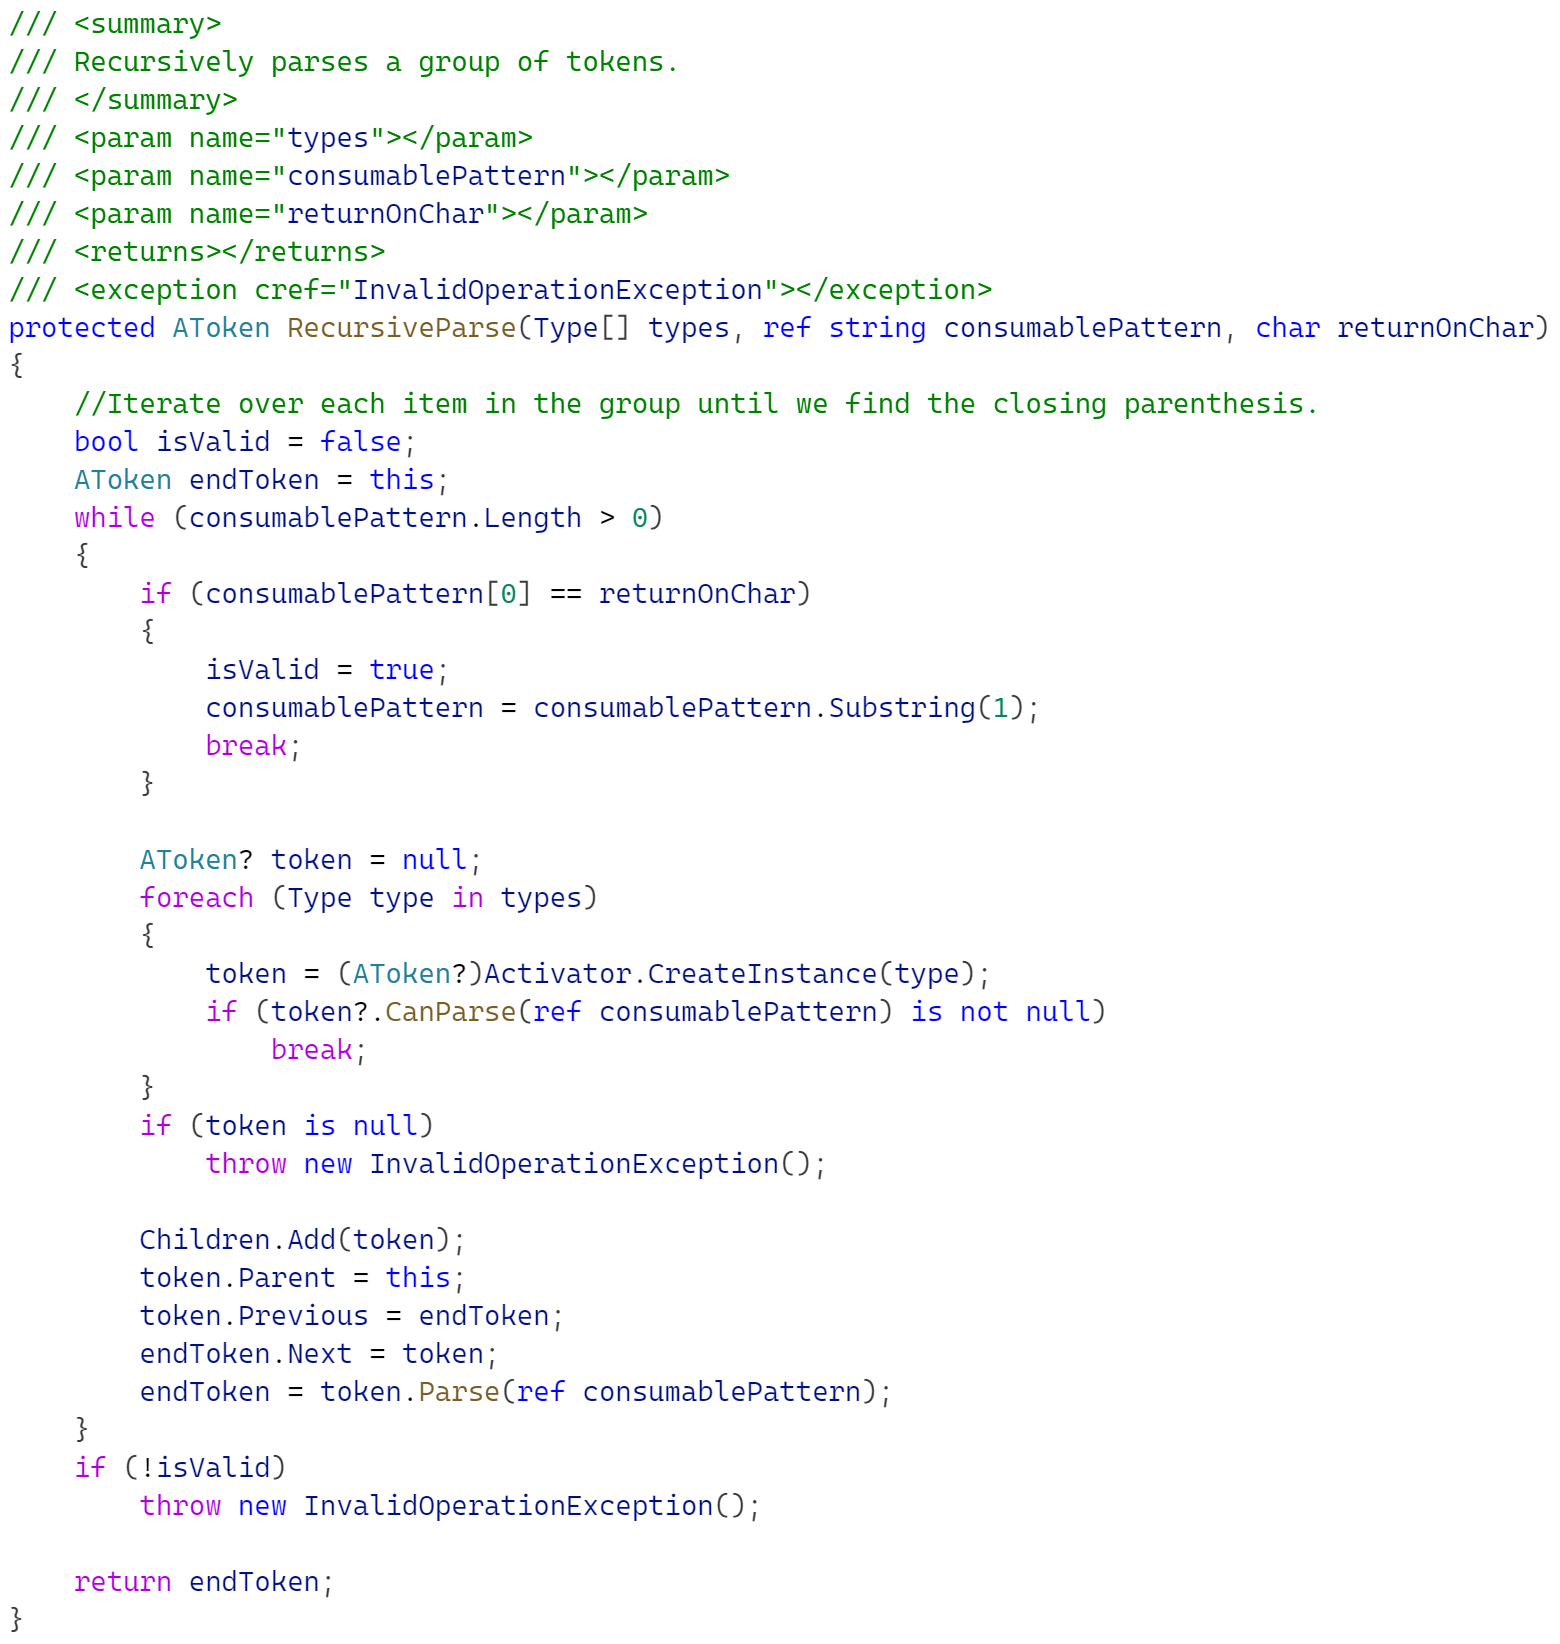
\includegraphics[width=\linewidth, height=\textheight, keepaspectratio]{Figures/AToken_RecursiveParse.png}
        \end{subfigure}
    \end{minipage}
    \begin{minipage}[t]{0.6\linewidth}
        % \vspace{-100px}
        \centering
        \caption{Character Range Conform}
        \label{fig:CharacterRangeConform}
        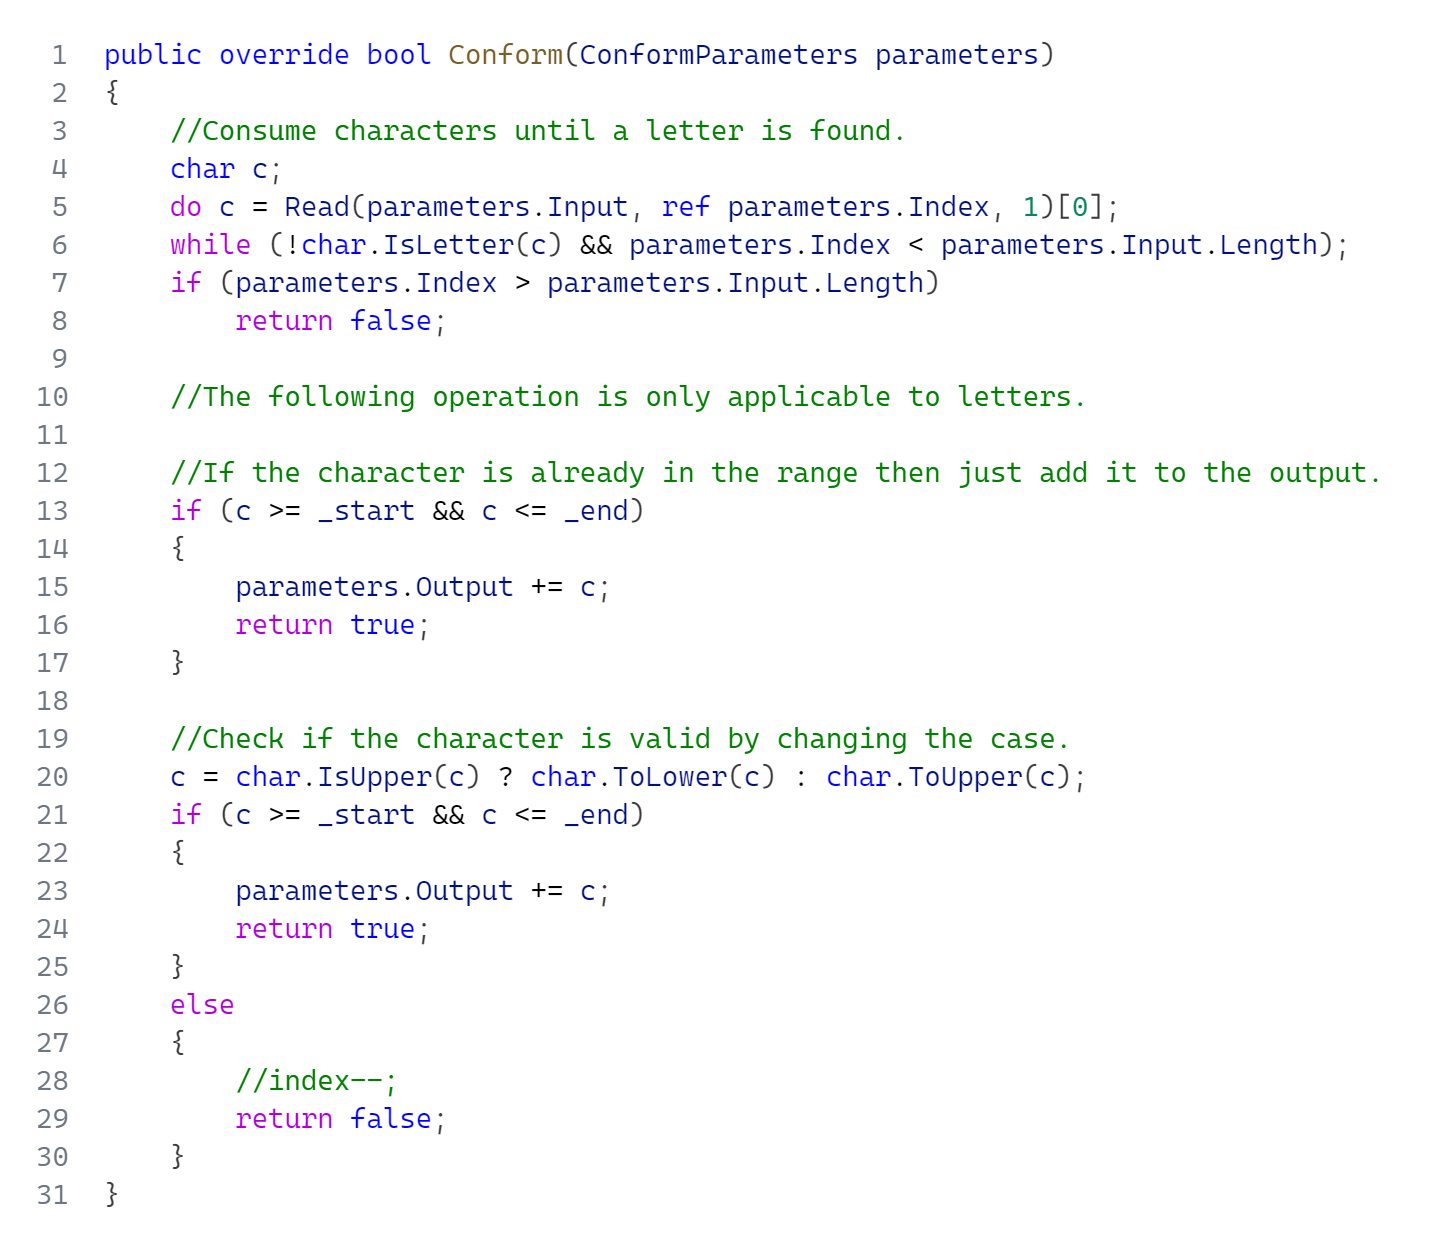
\includegraphics[width=0.95\textwidth]{Figures/CharacterRangeConform.png}
    \end{minipage}
}
\end{figure}

\begin{figure}
    \vspace{-50px}
    \centering
    \caption{VSIX Configuration manager}
    \label{fig:VSIXConfigurationManager}
    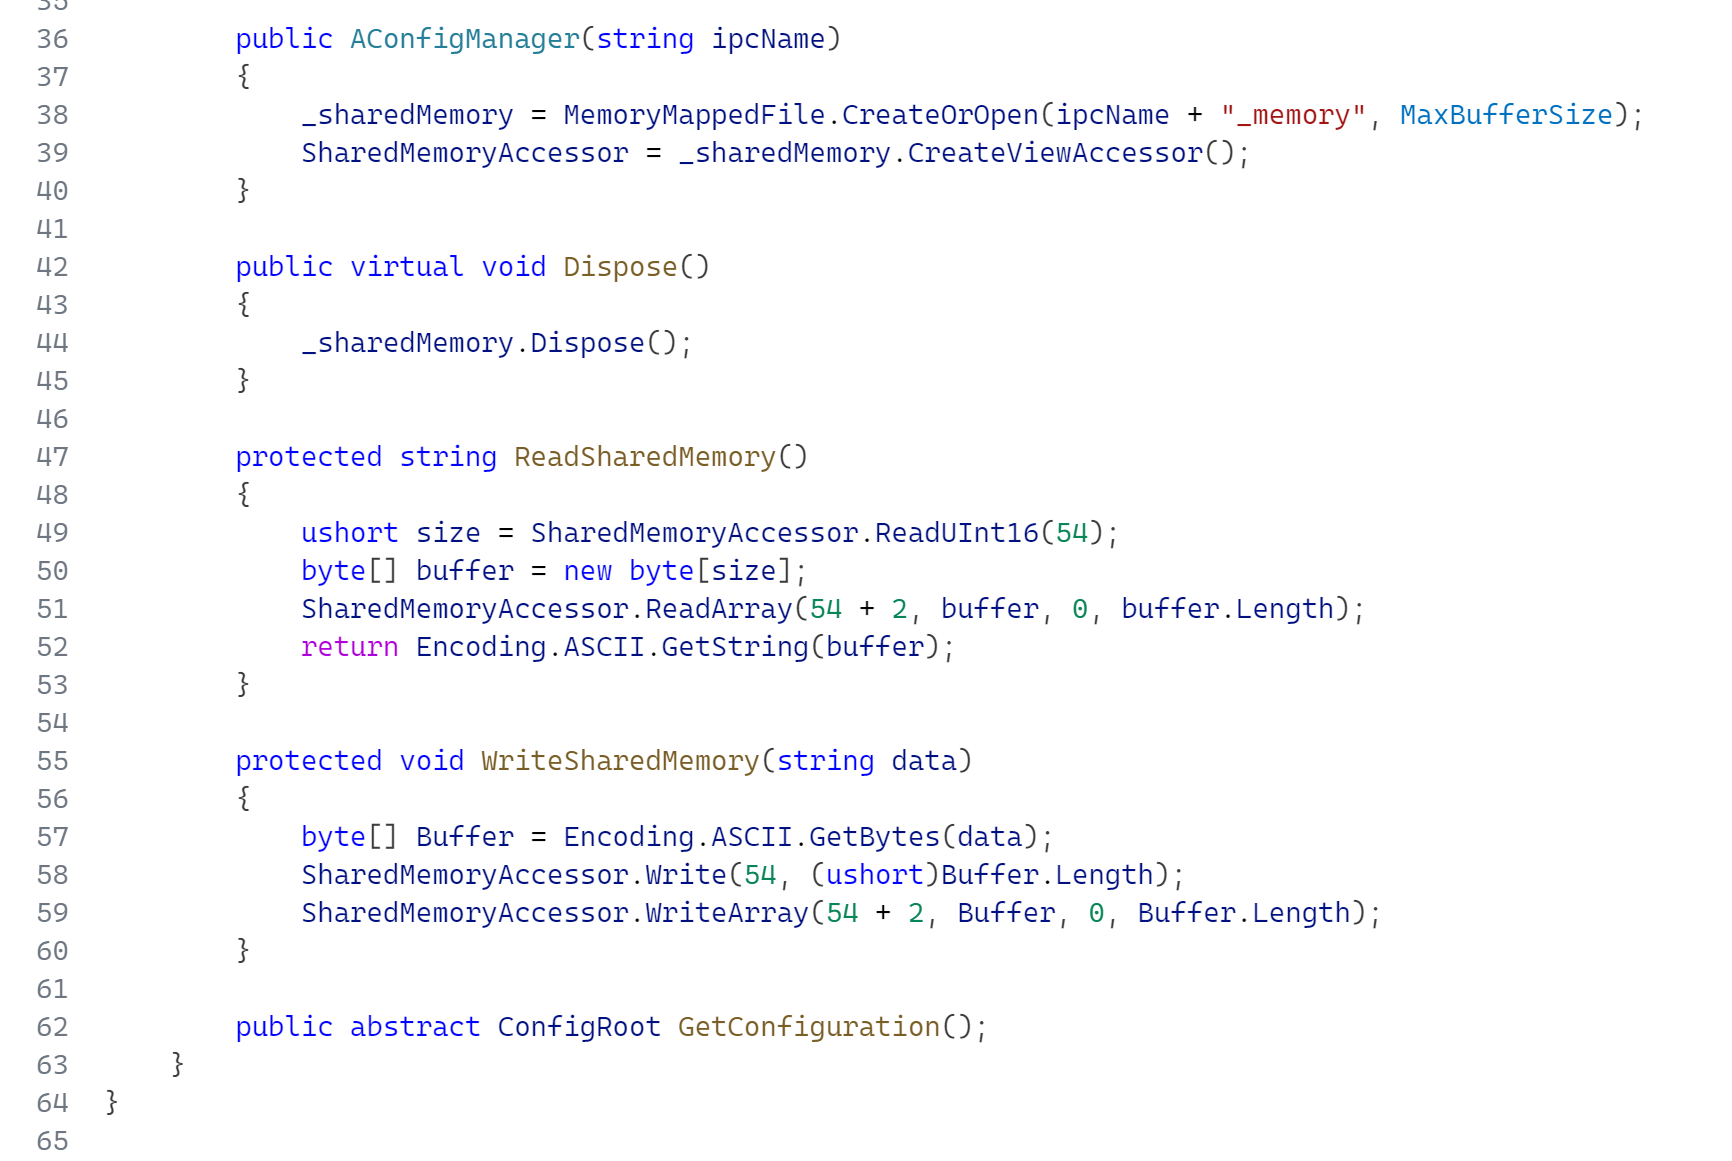
\includegraphics[width=0.8\textwidth]{Figures/VSIXAConfigManagerCropped.png}
\end{figure}

\begin{figure}[htp]
    % \vspace{-50px}
    \centering
    \caption{Quantifier Conform Parameters}
    \label{fig:QuantifierConformParameters}
    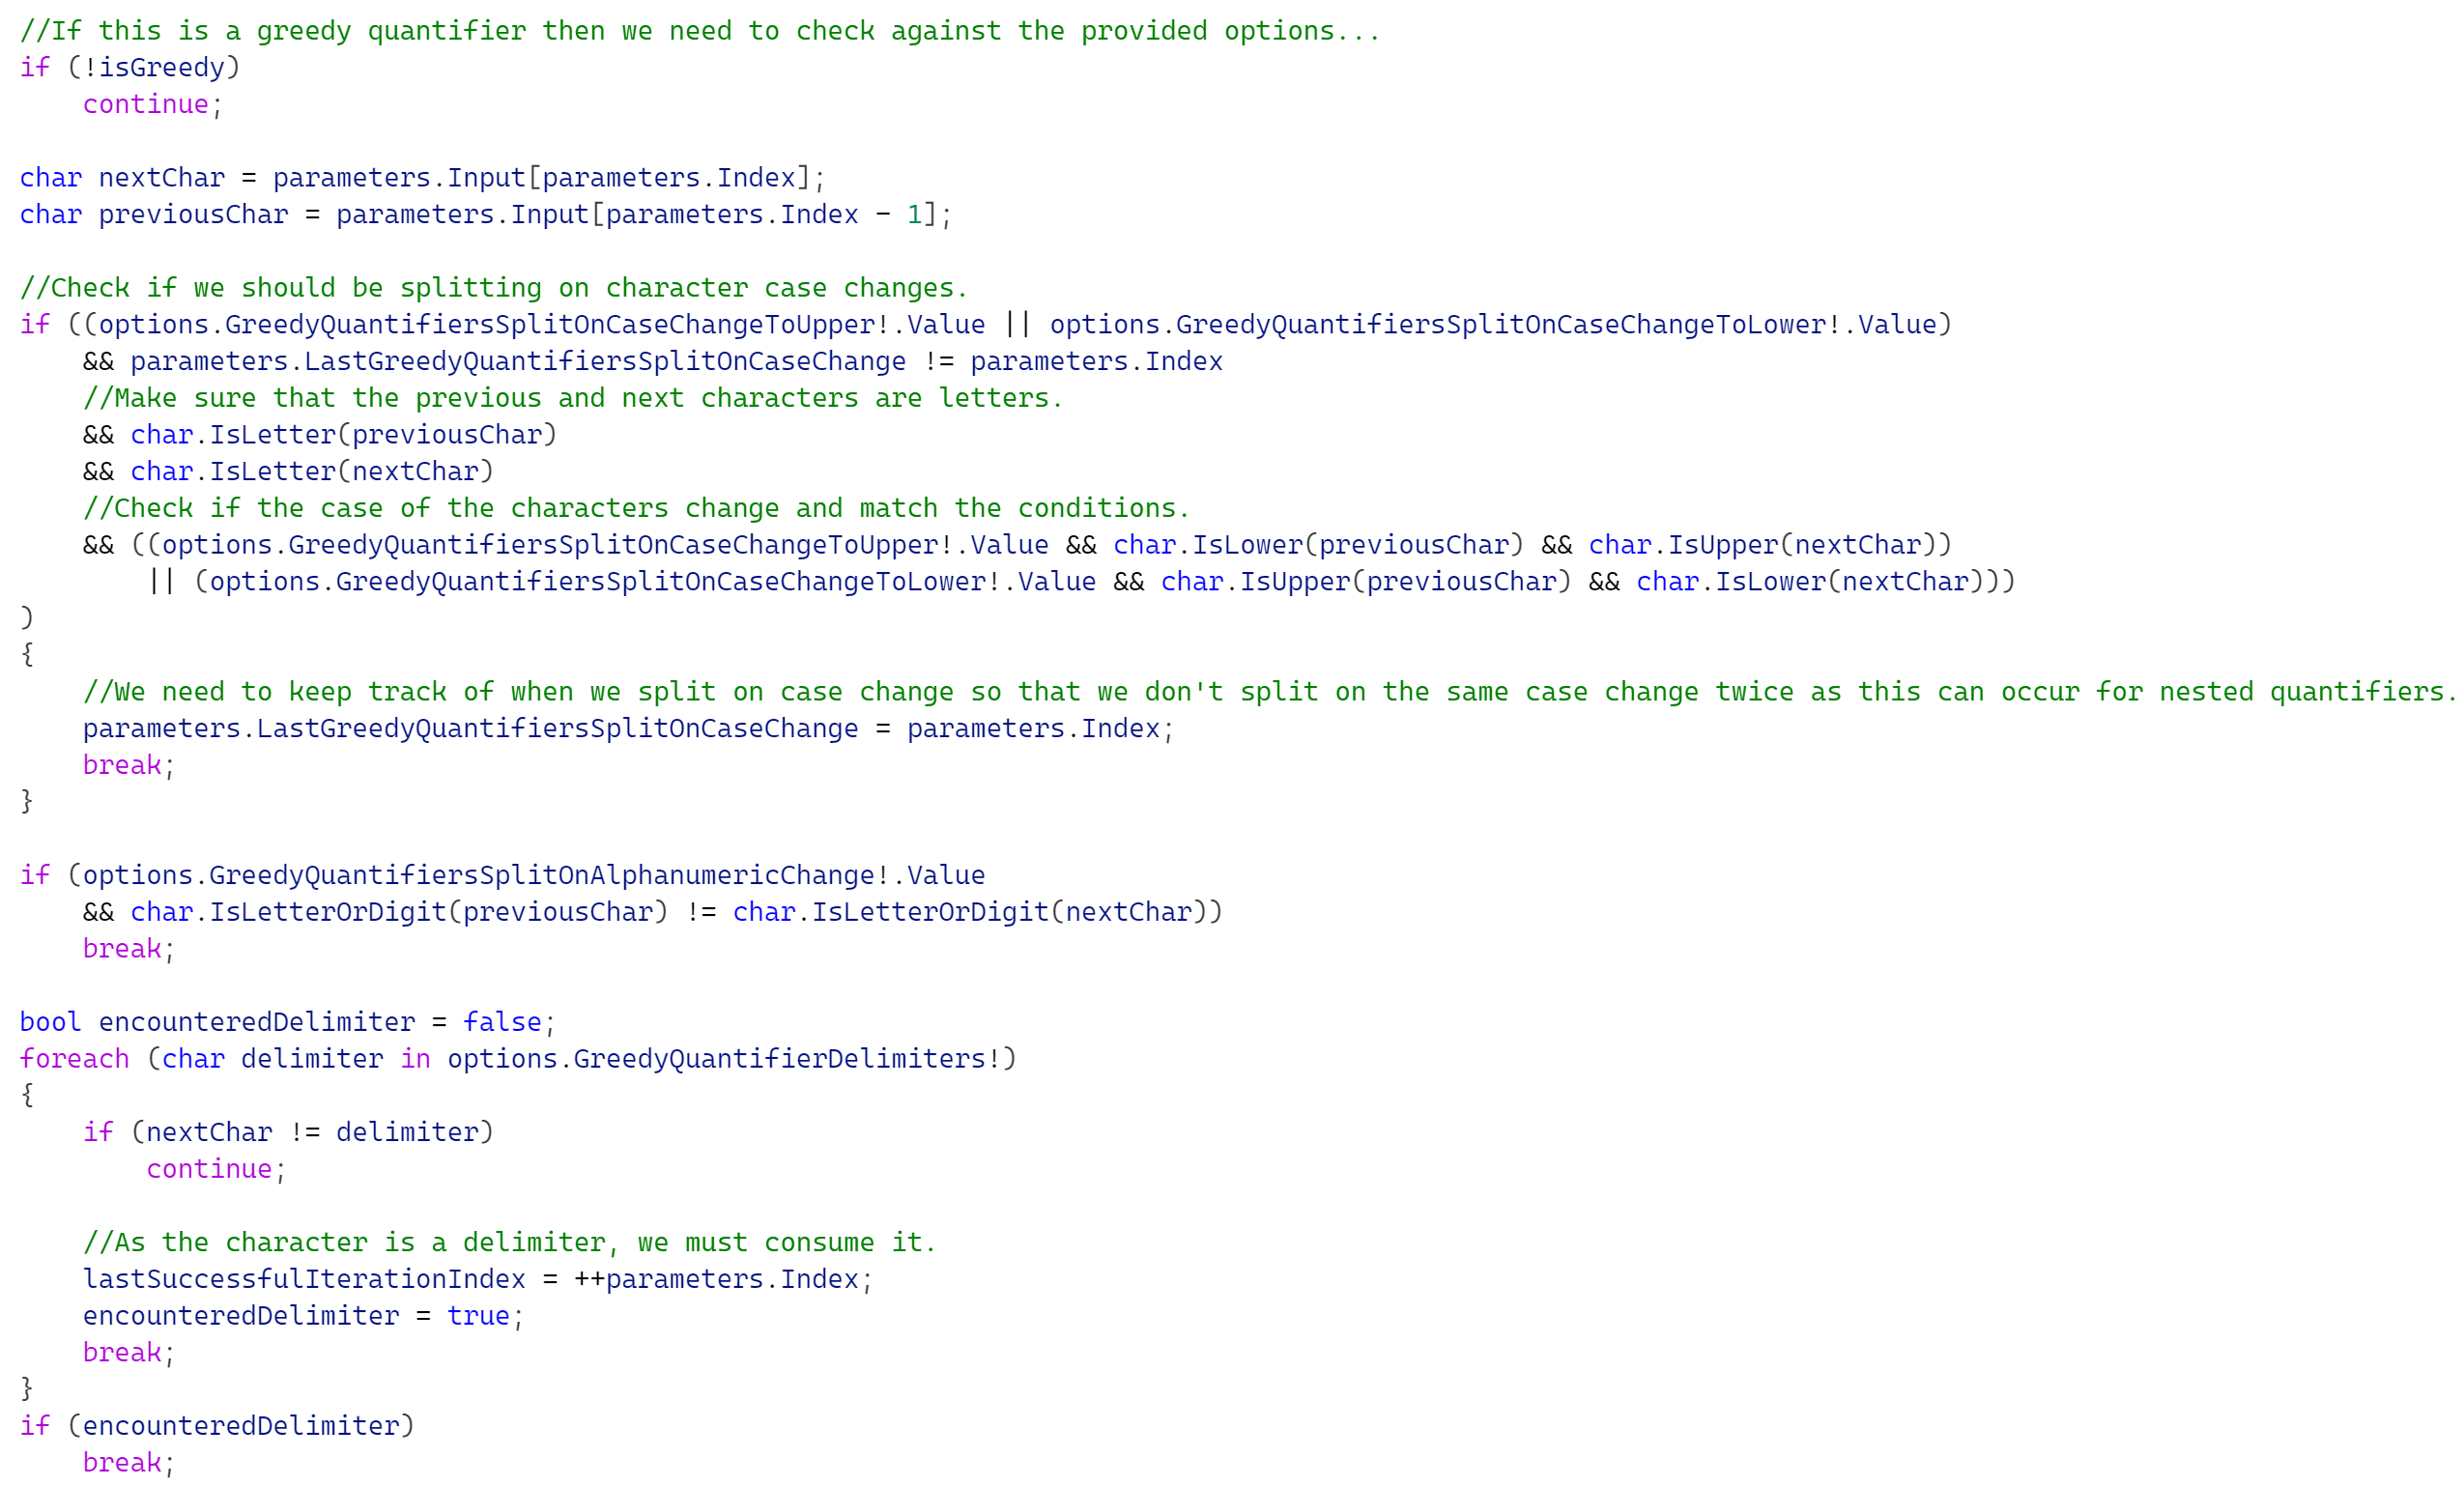
\includegraphics[width=1.0\textwidth]{Figures/QuantifierConformParameters.png}
\end{figure}

% \begin{figure}
%     \centering
%     \caption{Character Range Conform}
%     \label{fig:CharacterRangeConform}
%     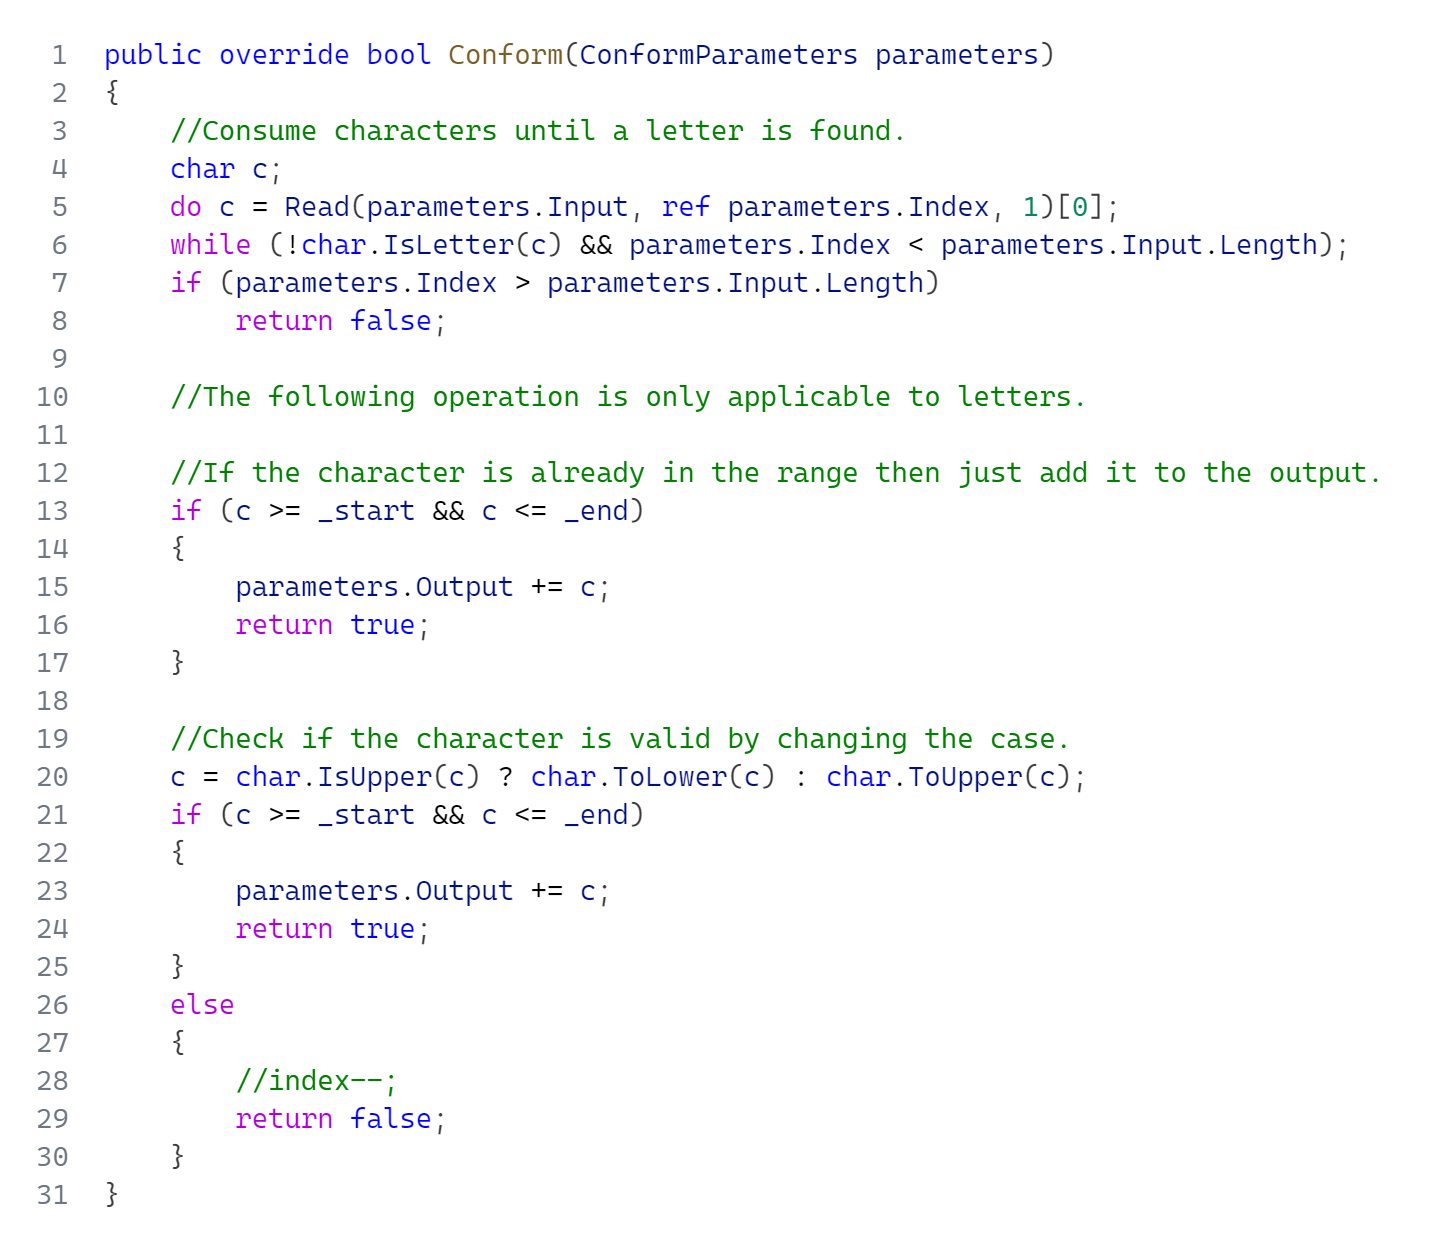
\includegraphics[width=0.5\textwidth]{Figures/CharacterRangeConform.png}
% \end{figure}

% \newpage
% % \begin{figure}[htbp]
% \begin{figure}
%     \centering
%     \begin{minipage}[b]{0.45\linewidth}
%         \centering
%         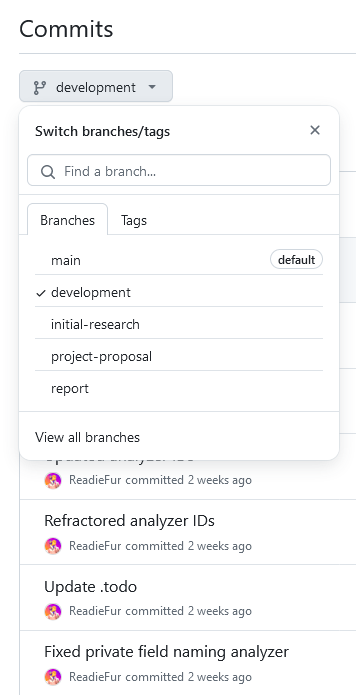
\includegraphics[width=\linewidth]{Figures/GitHubCommitHistoryCropped.png}
%         \caption{Caption for Image 1}
%         \label{fig:image1}
%     \end{minipage}
%     \hspace{0.5cm}
%     \begin{minipage}[b]{0.45\linewidth}
%         \centering
%         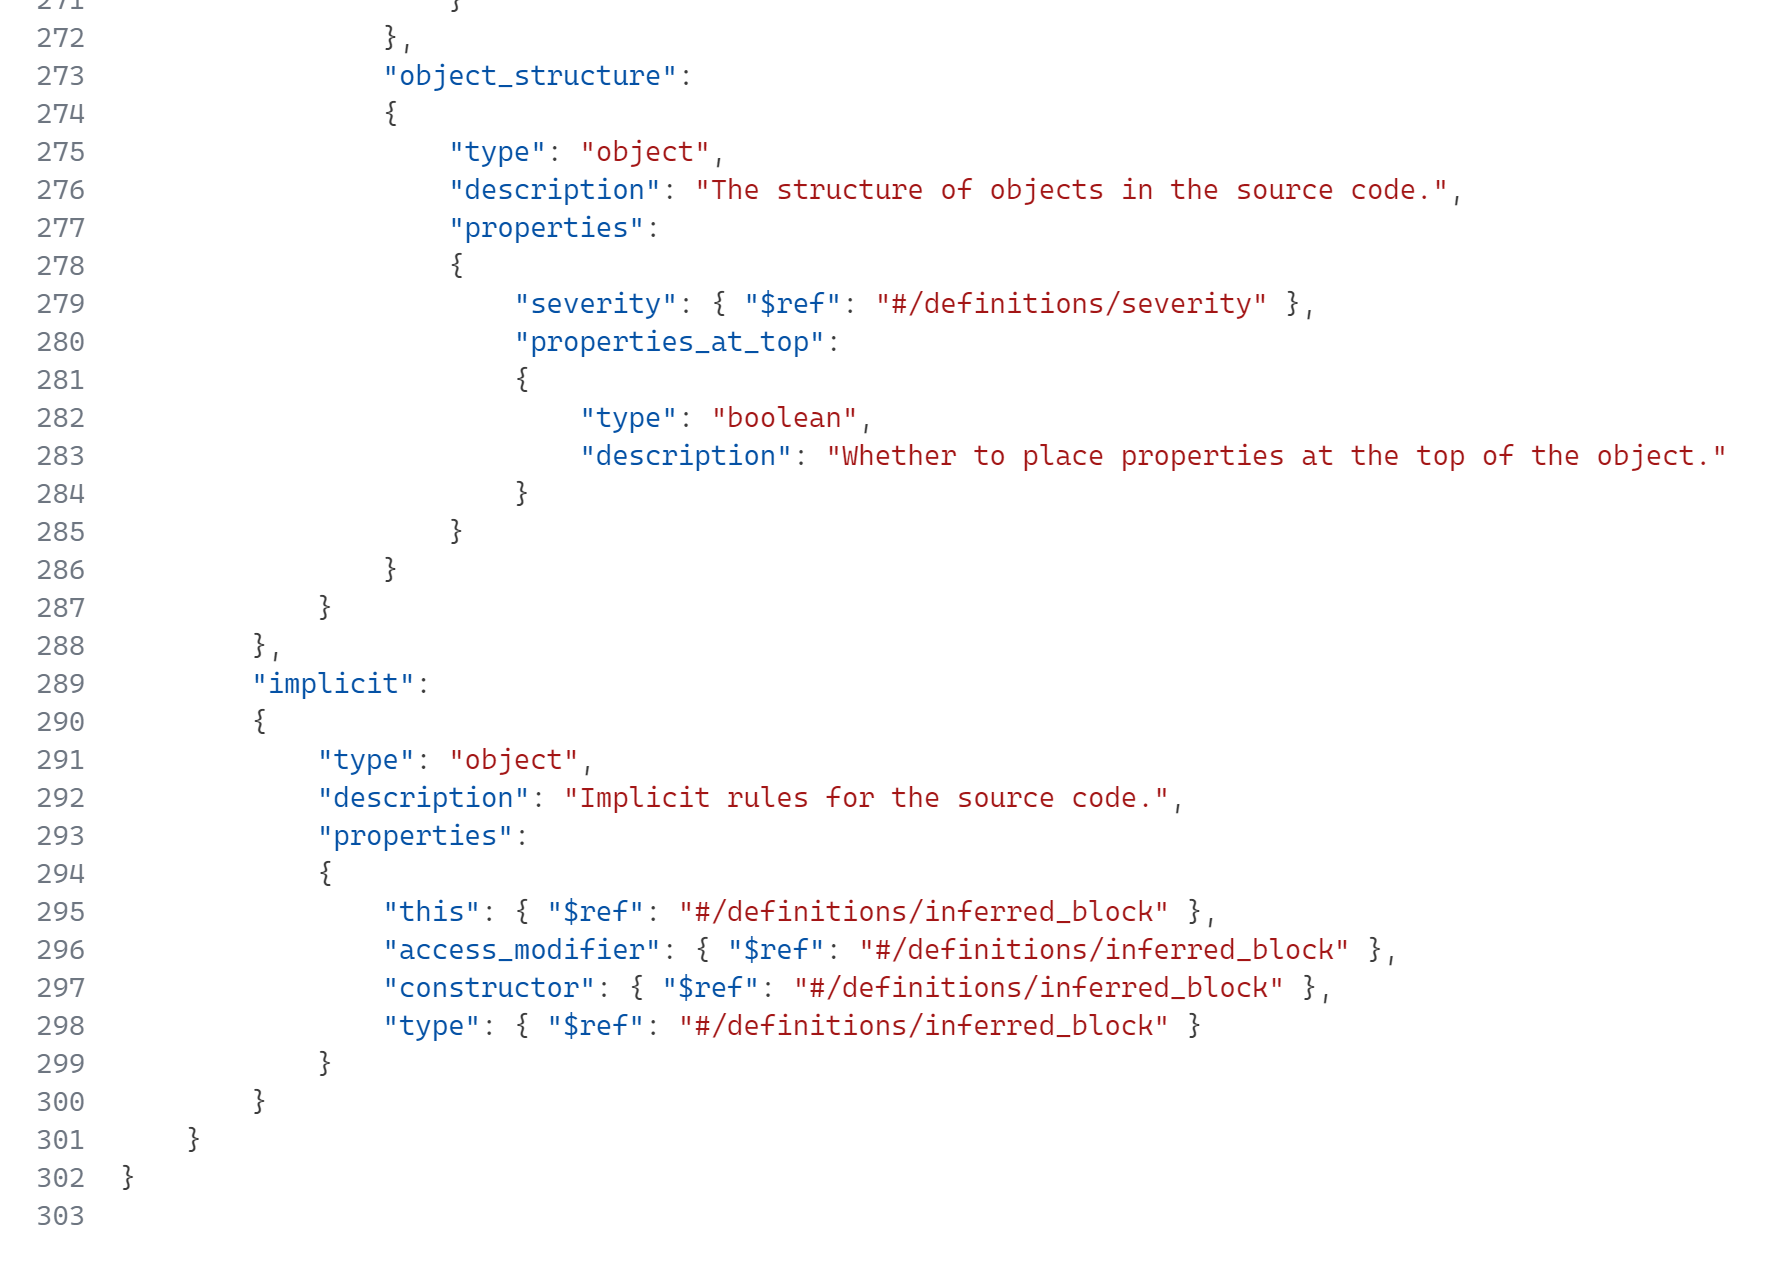
\includegraphics[width=\linewidth]{Figures/YAMLSchemaCropped.png}
%         \caption{Caption for Image 2}
%         \label{fig:image2}
%     \end{minipage}
% \end{figure}
% \begin{figure}[htbp]
% \centering
% \makebox[\textwidth][c]{%
%     \begin{minipage}[b]{0.7\linewidth}
%         \centering
%         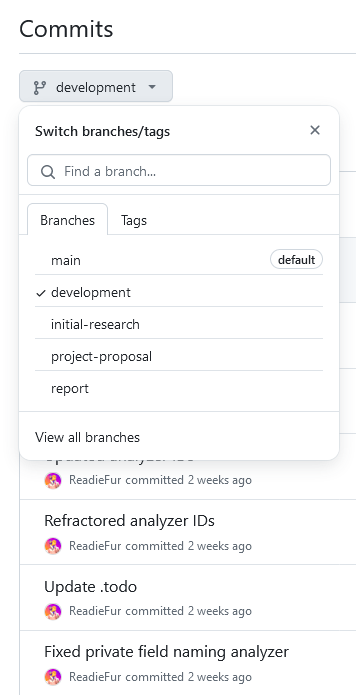
\includegraphics[width=\linewidth]{Figures/GitHubCommitHistoryCropped.png}
%         \caption{Caption for Image 1}
%         \label{fig:image1}
%     \end{minipage}%
%     \hspace{0.05\linewidth}% Adjust the spacing between figures
%     \begin{minipage}[b]{0.45\linewidth}
%         \centering
%         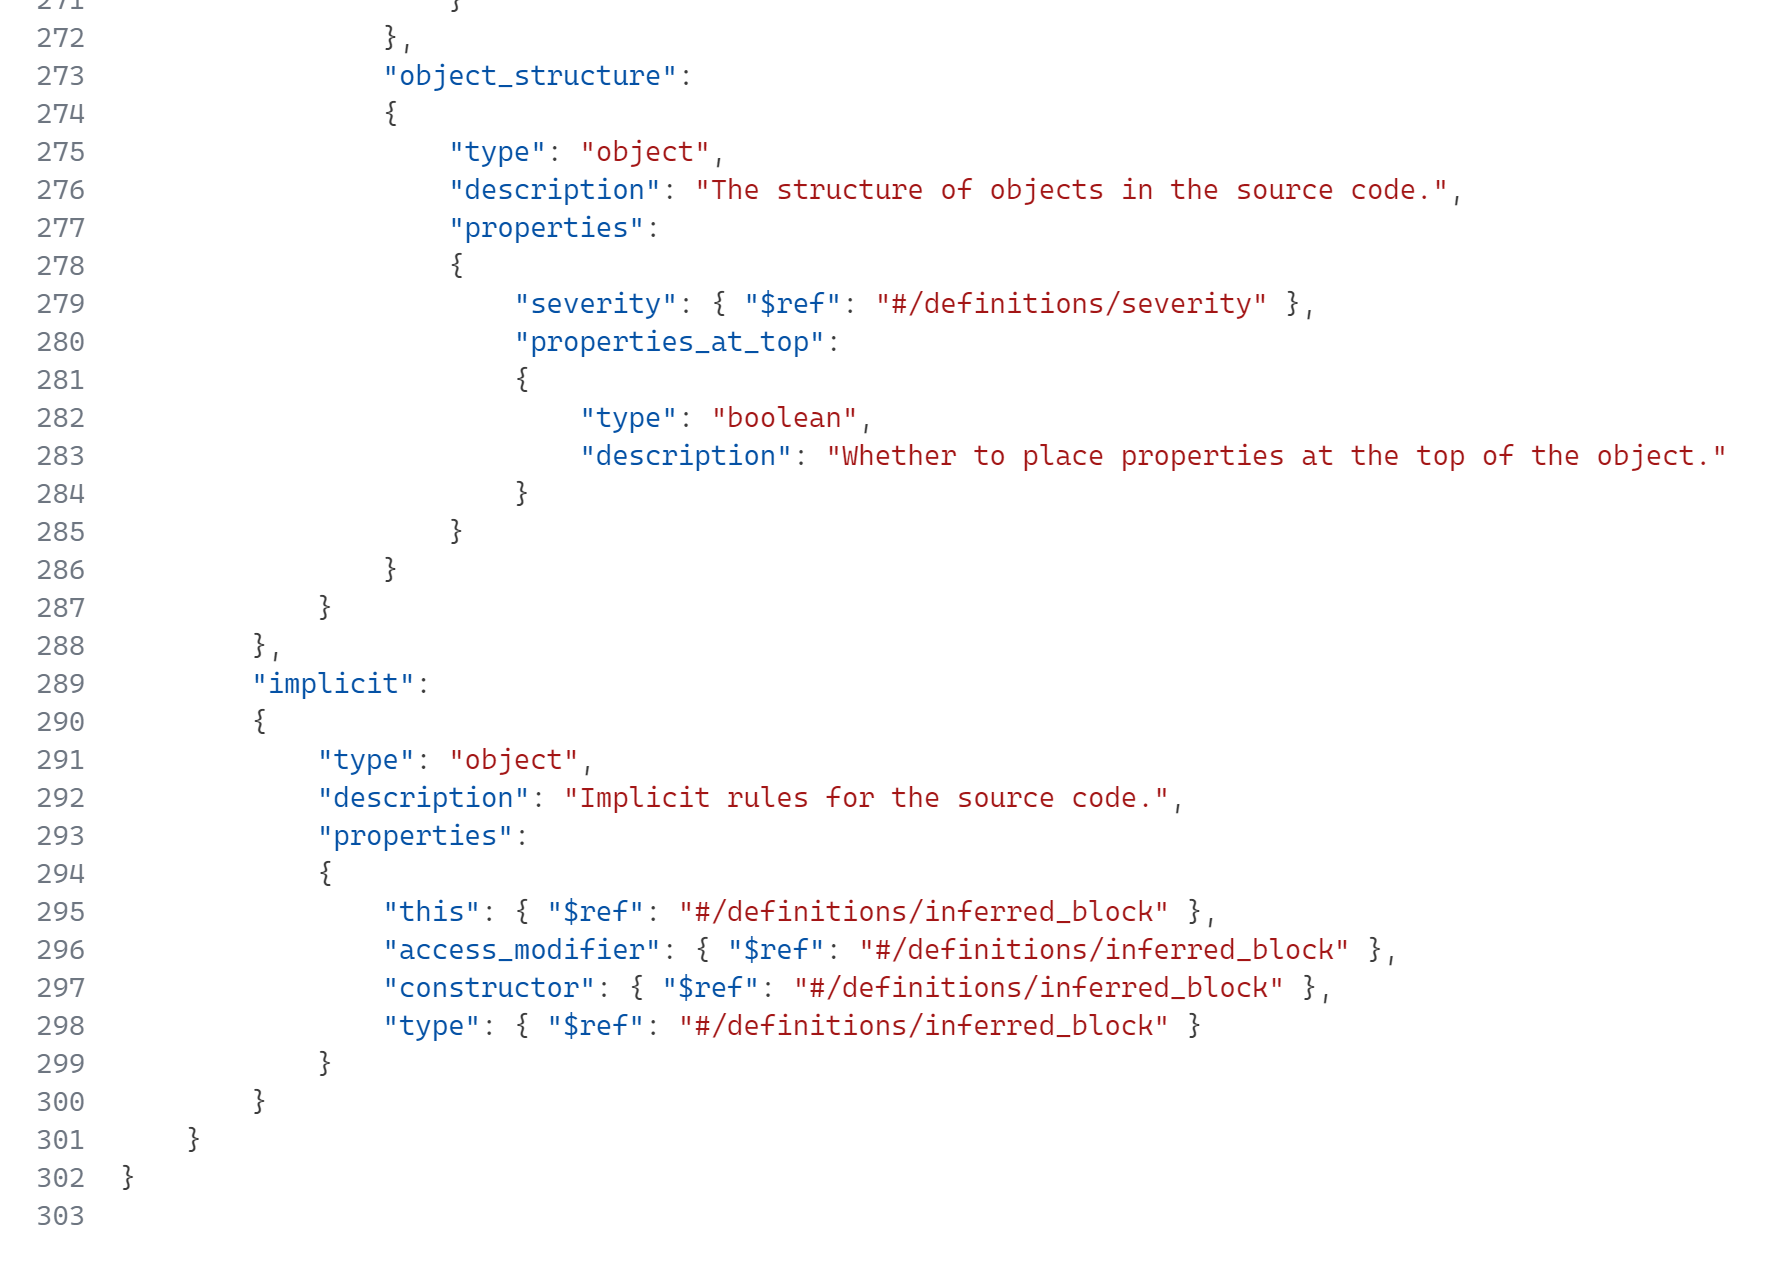
\includegraphics[width=\linewidth]{Figures/YAMLSchemaCropped.png}
%         \caption{Caption for Image 2}
%         \label{fig:image2}
%     \end{minipage}%
% }
% \end{figure}
